% Options for packages loaded elsewhere
% Options for packages loaded elsewhere
\PassOptionsToPackage{unicode}{hyperref}
\PassOptionsToPackage{hyphens}{url}
\PassOptionsToPackage{dvipsnames,svgnames,x11names}{xcolor}
%
\documentclass[
  letterpaper,
  DIV=11,
  numbers=noendperiod]{scrartcl}
\usepackage{xcolor}
\usepackage[top=4cm,bottom=4cm,left=3cm,right=3cm]{geometry}
\usepackage{amsmath,amssymb}
\setcounter{secnumdepth}{-\maxdimen} % remove section numbering
\usepackage{iftex}
\ifPDFTeX
  \usepackage[T1]{fontenc}
  \usepackage[utf8]{inputenc}
  \usepackage{textcomp} % provide euro and other symbols
\else % if luatex or xetex
  \usepackage{unicode-math} % this also loads fontspec
  \defaultfontfeatures{Scale=MatchLowercase}
  \defaultfontfeatures[\rmfamily]{Ligatures=TeX,Scale=1}
\fi
\usepackage{lmodern}
\ifPDFTeX\else
  % xetex/luatex font selection
\fi
% Use upquote if available, for straight quotes in verbatim environments
\IfFileExists{upquote.sty}{\usepackage{upquote}}{}
\IfFileExists{microtype.sty}{% use microtype if available
  \usepackage[]{microtype}
  \UseMicrotypeSet[protrusion]{basicmath} % disable protrusion for tt fonts
}{}
% Make \paragraph and \subparagraph free-standing
\makeatletter
\ifx\paragraph\undefined\else
  \let\oldparagraph\paragraph
  \renewcommand{\paragraph}{
    \@ifstar
      \xxxParagraphStar
      \xxxParagraphNoStar
  }
  \newcommand{\xxxParagraphStar}[1]{\oldparagraph*{#1}\mbox{}}
  \newcommand{\xxxParagraphNoStar}[1]{\oldparagraph{#1}\mbox{}}
\fi
\ifx\subparagraph\undefined\else
  \let\oldsubparagraph\subparagraph
  \renewcommand{\subparagraph}{
    \@ifstar
      \xxxSubParagraphStar
      \xxxSubParagraphNoStar
  }
  \newcommand{\xxxSubParagraphStar}[1]{\oldsubparagraph*{#1}\mbox{}}
  \newcommand{\xxxSubParagraphNoStar}[1]{\oldsubparagraph{#1}\mbox{}}
\fi
\makeatother


\usepackage{longtable,booktabs,array}
\usepackage{calc} % for calculating minipage widths
% Correct order of tables after \paragraph or \subparagraph
\usepackage{etoolbox}
\makeatletter
\patchcmd\longtable{\par}{\if@noskipsec\mbox{}\fi\par}{}{}
\makeatother
% Allow footnotes in longtable head/foot
\IfFileExists{footnotehyper.sty}{\usepackage{footnotehyper}}{\usepackage{footnote}}
\makesavenoteenv{longtable}
\usepackage{graphicx}
\makeatletter
\newsavebox\pandoc@box
\newcommand*\pandocbounded[1]{% scales image to fit in text height/width
  \sbox\pandoc@box{#1}%
  \Gscale@div\@tempa{\textheight}{\dimexpr\ht\pandoc@box+\dp\pandoc@box\relax}%
  \Gscale@div\@tempb{\linewidth}{\wd\pandoc@box}%
  \ifdim\@tempb\p@<\@tempa\p@\let\@tempa\@tempb\fi% select the smaller of both
  \ifdim\@tempa\p@<\p@\scalebox{\@tempa}{\usebox\pandoc@box}%
  \else\usebox{\pandoc@box}%
  \fi%
}
% Set default figure placement to htbp
\def\fps@figure{htbp}
\makeatother


% definitions for citeproc citations
\NewDocumentCommand\citeproctext{}{}
\NewDocumentCommand\citeproc{mm}{%
  \begingroup\def\citeproctext{#2}\cite{#1}\endgroup}
\makeatletter
 % allow citations to break across lines
 \let\@cite@ofmt\@firstofone
 % avoid brackets around text for \cite:
 \def\@biblabel#1{}
 \def\@cite#1#2{{#1\if@tempswa , #2\fi}}
\makeatother
\newlength{\cslhangindent}
\setlength{\cslhangindent}{1.5em}
\newlength{\csllabelwidth}
\setlength{\csllabelwidth}{3em}
\newenvironment{CSLReferences}[2] % #1 hanging-indent, #2 entry-spacing
 {\begin{list}{}{%
  \setlength{\itemindent}{0pt}
  \setlength{\leftmargin}{0pt}
  \setlength{\parsep}{0pt}
  % turn on hanging indent if param 1 is 1
  \ifodd #1
   \setlength{\leftmargin}{\cslhangindent}
   \setlength{\itemindent}{-1\cslhangindent}
  \fi
  % set entry spacing
  \setlength{\itemsep}{#2\baselineskip}}}
 {\end{list}}
\usepackage{calc}
\newcommand{\CSLBlock}[1]{\hfill\break\parbox[t]{\linewidth}{\strut\ignorespaces#1\strut}}
\newcommand{\CSLLeftMargin}[1]{\parbox[t]{\csllabelwidth}{\strut#1\strut}}
\newcommand{\CSLRightInline}[1]{\parbox[t]{\linewidth - \csllabelwidth}{\strut#1\strut}}
\newcommand{\CSLIndent}[1]{\hspace{\cslhangindent}#1}



\setlength{\emergencystretch}{3em} % prevent overfull lines

\providecommand{\tightlist}{%
  \setlength{\itemsep}{0pt}\setlength{\parskip}{0pt}}



 


\usepackage{booktabs}
\usepackage{longtable}
\usepackage{array}
\usepackage{multirow}
\usepackage{wrapfig}
\usepackage{float}
\usepackage{colortbl}
\usepackage{pdflscape}
\usepackage{tabu}
\usepackage{threeparttable}
\usepackage{threeparttablex}
\usepackage[normalem]{ulem}
\usepackage{makecell}
\usepackage{xcolor}
\KOMAoption{captions}{tableheading}
\makeatletter
\@ifpackageloaded{caption}{}{\usepackage{caption}}
\AtBeginDocument{%
\ifdefined\contentsname
  \renewcommand*\contentsname{Table of contents}
\else
  \newcommand\contentsname{Table of contents}
\fi
\ifdefined\listfigurename
  \renewcommand*\listfigurename{List of Figures}
\else
  \newcommand\listfigurename{List of Figures}
\fi
\ifdefined\listtablename
  \renewcommand*\listtablename{List of Tables}
\else
  \newcommand\listtablename{List of Tables}
\fi
\ifdefined\figurename
  \renewcommand*\figurename{Figure}
\else
  \newcommand\figurename{Figure}
\fi
\ifdefined\tablename
  \renewcommand*\tablename{Table}
\else
  \newcommand\tablename{Table}
\fi
}
\@ifpackageloaded{float}{}{\usepackage{float}}
\floatstyle{ruled}
\@ifundefined{c@chapter}{\newfloat{codelisting}{h}{lop}}{\newfloat{codelisting}{h}{lop}[chapter]}
\floatname{codelisting}{Listing}
\newcommand*\listoflistings{\listof{codelisting}{List of Listings}}
\makeatother
\makeatletter
\makeatother
\makeatletter
\@ifpackageloaded{caption}{}{\usepackage{caption}}
\@ifpackageloaded{subcaption}{}{\usepackage{subcaption}}
\makeatother
\usepackage{bookmark}
\IfFileExists{xurl.sty}{\usepackage{xurl}}{} % add URL line breaks if available
\urlstyle{same}
\hypersetup{
  colorlinks=true,
  linkcolor={blue},
  filecolor={Maroon},
  citecolor={Blue},
  urlcolor={Blue},
  pdfcreator={LaTeX via pandoc}}


\author{}
\date{}
\begin{document}


\begin{titlepage}
\centering
\vspace*{3cm}

{\Huge Busy Making Other Plans:\par}
\vspace{0.8cm}

{\Large \bfseries A Simulation Study on the Effects of Deviations from Preregistrations\par}
\vspace{1cm}

{\large A. J. Vijlbrief\par}
{\large May 11, 2026\par}

\vfill

{\large\textbf{Supervisors}\par}
A. M. Scheel\\
H. I. Oberman

\vspace{0.5cm}

{\large\textbf{Word Count}\par}
idkyet
\end{titlepage}

The inability to reliably reproduce findings in the field of psychology
is a known problem. The Open Science Collaboration (2015) found that
only 36\% of significant results were reproducible. One reason for this
``replication crisis'' is ``researcher degrees of freedom'' (Simmons et
al., 2011). This term describes the flexibility that researchers have in
decisions made during their work. This includes decisions such as how
many observations to collect, which statistical model to use and which
covariates to add. When these decisions are made during data collection
or analysis, researchers can make opportunistic choices which steer
their results towards desired outcomes. Such opportunistic choices are
called \emph{p}-hacking and can dramatically increase false-positive
rates (Stefan \& Schönbrodt, 2023).

The preregistration was proposed as a way to limit these types of
practices. Preregistrations are documents that are published at the
start of the research process, in which decisions concerning data
collection and analysis are recorded. Templates are available to
researchers, to inform them about what information is important to
preregister. The preregistration is then uploaded to a public
repository, with a time stamp of when it was published. Peer reviewers,
and others, have access to the preregistration and can evaluate it
before the start of the study or compare it to the final research paper.
This practice increases transparency about research choices and has
become more popular, with the number of preregistrations increasing
annually (Ferguson et al., 2023; Lindsay et al., 2018).

In theory preregistration works well, if researchers are specific in
their preregistration and follow it closely, this should lead to better
reproducible findings. In practice, preregistrations are often imprecise
and incomplete, making them less effective at restricting researcher
degrees of freedom. Furthermore, no difference has been found between
preregistered and non-preregistered papers in the number of significant
findings (van den Akker, van Assen, et al., 2024), and no reduction in
\emph{p}-hacking (Brodeur et al., 2024).

Another common problem are deviations from preregistration (Claesen et
al., 2021; van den Akker, Bakker, et al., 2024). Deviating means that
the preregistered plan is not being followed during the execution of the
study. Deviations have been found in as many as 93\% of preregistered
papers, with up to 89\% being incompletely reported (Claesen et al.,
2021; Willroth \& Atherton, 2024). These changes occur most commonly in
data collection procedures, statistical models and exclusion criteria
(van den Akker, Bakker, et al., 2024). This includes differences in the
total sample size, how outliers are selected and which covariates are
used. These deviations could serve to further diminish the effectiveness
of preregistrations, as it reintroduces researcher degrees of freedom
and leaves room to revert back to \emph{p}-hacking strategies.

\subsubsection{Are all deviations bad?}\label{are-all-deviations-bad}

Deviations from preregistrations occur in all different aspects of the
research process, but what is not known is the effect of these
deviations. Do changes from original research plans reduce research
quality? Lakens (2024) theorized what the possible consequences could
be. If deviations occur due to assumptions being violated or data no
longer being suitable for the planned analysis, then deviating from the
original research plan can have positive effects on the validity of a
test. Similarly, adding additional analyses can increase the robustness.
On the other hand, changes in testing also mean that a hypothesis is
generally less ``severely'' tested. This means that a theory has not
been given the proper opportunity to be falsified which can result in
higher type II errors. Consequently, little can be said about whether
deviations are bad, especially when the reason for the deviation is
unknown.

There is no clear consensus on whether inconsistencies between
preregistrations and final publications are a problem. When asked,
researchers themselves deemed deviations to be problematic to varying
degrees (Willroth \& Atherton, 2024). Changes to analyses and hypotheses
were considered the least acceptable, whereas changing research
platforms or software were deemed relatively justifiable. The estimated
impact on the results and whether the deviation was reported
transparently and were also taken into consideration. To summarize, even
though deviations from preregistration are common, a clear conclusion on
their effects is still missing.

\subsubsection{The present project}\label{the-present-project}

With this simulation study, I intend to close this gap in the literature
and explore the effects of typical preregistration deviations on
research outcomes and the quality of published results. Specifically, I
aim to answer the question: `How do deviations from preregistrations
affect type I and type II error rates?' The effect of deviations is
studied in three domains: sample size, outlier exclusion criteria, and
the statistical model. Different deviations are simulated in each domain
and compared to a baseline condition without deviations. This research
question is investigated in the context of social sciences and uses a
linear regression as the model of interest. The effects are examined
across two scenarios: a no-effect scenario, and an effect scenario, in
which the main effect parameter is changed. The aim of this study is
descriptive and therefore no specific hypotheses are formulated.

As a secondary research question, I address the issue of reasons for
deviations being unknown. The reason behind a deviation is important for
assessing its effect. A researcher being forced to deviate due to
circumstance is very different from a researcher \emph{choosing} to
deviate. When a researcher chooses to deviate, this could be because
they are picking the results they prefer. Initially, the deviation
conditions are simulated and the outcomes are used to assess type I and
type II error as compared to the baseline condition. For the second
research question, an `opportunistic' condition is created in which
outcomes are selectively chosen from either the baseline or the
deviation conditions, based on which condition has a significant
\emph{p}-value. This is done in order to proxy the opportunistic
selection of results by the researcher.

With these simulations I hope to shed light on the effect of deviations
from preregistration on type I and type II errors, as well as the effect
of picking deviations opportunistically.

\subsection{Methods}\label{methods}

\subsubsection{Conditions}\label{conditions}

I reviewed which deviations to investigate by (1) how common they are,
(2) their potential impact and (3) their justifiability. Based on this,
deviations were chosen in the following domains: sample size, outlier
exclusion criteria, and statistical model. Within the three chosen
domains, multiple conditions were simulated and compared to a baseline
condition without any deviations.

\paragraph{Sample size}\label{sample-size}

Deviations in the sample size are some of the most common deviations,
with consistency between preregistrations and published papers only
being 28\% for the exact sample size (van den Akker, Bakker, et al.,
2024). Changing the sample size can inflate type II error (by decreasing
power) as well as the type I error (Lakens, 2024; Simmons et al., 2011).
Small deviations in sample size are common and often due to factors
outside of the researcher's agency. Researchers also admit to stopping
collection earlier or continuing collection longer after finding
disappointing results (John et al., 2012). However, it is unknown how
often this is also used as a reason to deviate from preregistrations.
Based on this, the conditions in Table~\ref{tbl-cond} are simulated
within the sample size domain.

\paragraph{Outlier exclusion criteria}\label{outlier-exclusion-criteria}

Literature shows that over half of published papers do not adhere to
their pre-specified outlier exclusion criteria (Claesen et al., 2021;
van den Akker, Bakker, et al., 2024). Vague or missing criteria in
preregistrations make it harder to assess deviations and leave a lot of
room for interpretation and ad hoc decisions (Heirene et al., 2024).
This could potentially lead researchers to choose how to exclude
outliers based on which method provides better results. Researchers
themselves, however, deem outlier deviations to be relatively acceptable
(Willroth \& Atherton, 2024).

Lakens (2024) argues that adding additional exclusion criteria can
undermine the severity of a test. This idea is corroborated by Stefan \&
Schönbrodt (2023), who showed that the type I error increases linearly
with the number of outlier detection methods used. Furthermore, 38\% of
researchers admit to excluding outliers only after examining their
impact on the data (John et al., 2012). If this is also the reason why
many people deviate from their preregistered outlier criteria, then
these deviations are important.

The most common method for identifying outliers in the social sciences
is the \emph{z}-score (Bakker \& Wicherts, 2014; Leys et al., 2013). A
minimum of three standard deviations from the mean is often maintained
as the rule of thumb for excluding cases. Within linear regression,
outliers are also often identified based on their influence, commonly
using Cook's distance. Cook's distance excludes outliers based on how
much their exclusion would influence the regression coefficients. In
this study, the baseline condition will be to exclude datapoints based
on a \emph{z}-score of 3 standard deviations from the mean, with
deviation conditions based on a stricter \emph{z}-score and Cook's
distance (Table~\ref{tbl-cond}).

\paragraph{Statistical model}\label{statistical-model}

Amongst all of the aforementioned domains, the least is known about why
people deviate from their preregistered statistical model. ``Statistical
model'' is a very broad domain and includes many types of deviations,
such as changes in the dependent variable, independent variable,
statistical inference criteria and the actual statistical test. In this
paper, ``statistical model'' refers to the above-mentioned types of
changes, not only the statistical test and its specifications.

The broadness of the domain also means that deviations within the domain
have been investigated from multiple angles. Claesen et al. (2021) found
a deviation rate of 70\% within the ``analysis'' domain, including
deviations like examining additional effects, changing which model is
tested and performing unregistered robustness checks. The majority of
these deviations went unreported. Another study reported inconsistencies
in 40\% of the statistical models, deviations included the
specifications of the variables, which model was tested and how
variables were used (van den Akker, Bakker, et al., 2024).

As Lakens (2024) argues, at times it might be necessary to alter the
statistical model. This could happen when a variable has been measured
at a different level than expected or a test assumption has been
violated. However, changing the statistical model can also be done
opportunistically. Choosing to add an extra dependent variable because
results are not yet satisfying can increase the type I error rate to
9.5\%, and the addition of a covariate can increase it to 11.7\%
(Simmons et al., 2011). The reasoning behind the change thus becomes
very important. Therefore, deviations due to failing to properly specify
how variables would be operationalized in the preregistration are also
seen as a larger shortcoming than model deviations due to unforeseen
consequences (Willroth \& Atherton, 2024). Within the statistical model,
three deviation conditions are simulated: outcome switching, adding a
continuous covariate, and adding a dichotomous covariate
(Table~\ref{tbl-cond}).

\begin{longtable}[]{@{}
  >{\raggedright\arraybackslash}p{(\linewidth - 4\tabcolsep) * \real{0.4135}}
  >{\raggedright\arraybackslash}p{(\linewidth - 4\tabcolsep) * \real{0.2212}}
  >{\raggedright\arraybackslash}p{(\linewidth - 4\tabcolsep) * \real{0.3558}}@{}}
\caption{Parameter Values for Baseline Condition and Deviation
Conditions per Domain}\label{tbl-cond}\tabularnewline
\toprule\noalign{}
\begin{minipage}[b]{\linewidth}\raggedright
Domain
\end{minipage} & \begin{minipage}[b]{\linewidth}\raggedright
Baseline condition
\end{minipage} & \begin{minipage}[b]{\linewidth}\raggedright
Deviations conditions
\end{minipage} \\
\midrule\noalign{}
\endfirsthead
\toprule\noalign{}
\begin{minipage}[b]{\linewidth}\raggedright
Domain
\end{minipage} & \begin{minipage}[b]{\linewidth}\raggedright
Baseline condition
\end{minipage} & \begin{minipage}[b]{\linewidth}\raggedright
Deviations conditions
\end{minipage} \\
\midrule\noalign{}
\endhead
\bottomrule\noalign{}
\endlastfoot
Sample size & 200 & +5 \\
& & +30 \\
& & -5 \\
& & -30 \\
Outlier exclusion criteria &
\multicolumn{2}{>{\raggedright\arraybackslash}p{(\linewidth - 4\tabcolsep) * \real{0.5769} + 2\tabcolsep}@{}}{%
\emph{Z}-scores of 3 SD \textbar{} \emph{Z}-scores of 2 SD
\textbar{}} \\
& & Cook's distance of 1 \textbar{} \\
\multicolumn{3}{@{}>{\raggedright\arraybackslash}p{(\linewidth - 4\tabcolsep) * \real{0.9904} + 4\tabcolsep}@{}}{%
Statistical methods: covariates \textbar{} No covariates \textbar{}
Continuous covariate \textbar{} \textbar{} \textbar{} \textbar{}
\textbar{} Dichotomous covariate} \\
\multicolumn{3}{@{}>{\raggedright\arraybackslash}p{(\linewidth - 4\tabcolsep) * \real{0.9904} + 4\tabcolsep}@{}}{%
Statistical methods: outcome switching \textbar{} Y \textbar{} Ya
\textbar{}} \\
\end{longtable}

\emph{Note.} Variable Ya is defined in the next section.

\subsubsection{Data-generating
mechanism}\label{data-generating-mechanism}

Data is generated under two scenarios: ``X has an effect on Y'' and ``X
has no effect on Y''. The only difference in data generation between the
two scenarios is in the main effect parameter, \(\beta_1\). In the
effect scenario, \(\beta_1\) is 0.2, and in the no-effect scenario,
\(\beta_1\) is 0. In the baseline condition, the statistical model is
defined as \[
Y = \beta_0 + \beta_1X + \epsilon,
\] where \(Y\) is the dependent variable, \(\beta_0\) the intercept,
\(\beta_1\) the main effect, and \(\epsilon\) the random error.

The population parameter values are presented in Table~\ref{tbl-DGM},
together with the parameter values for the deviation conditions. The
complete data-generating model is defined as

\[
\begin{aligned}
Y &=  \beta_0 + \beta_1X + \beta_2Z + \beta_3D + \epsilon,\\
Y_a &\sim Y, \quad \rho(Y, Y_a) = 0.6, 
\end{aligned}
\]

where \(Z\) and \(D\) represent a continuous and categorical covariate
respectively and \(Y_a\) represents an alternative outcome variable with
a correlation of 0.6 with variable \(Y\).

As mentioned, data is generated under two scenarios: an effect scenario
and a no-effect scenario. The only difference in data generation between
the two scenarios is in the main effect parameter, \(\beta_1\).

In order to assess differences between outlier exclusion criteria, the
data needs to include outliers. These are simulated by generating 5\% of
the data, 2.5\% at each end of the distribution, with -3 and 3 as mean
values for the normal distribution from which \(\epsilon\) is drawn.

\begin{longtable}[]{@{}
  >{\raggedright\arraybackslash}p{(\linewidth - 2\tabcolsep) * \real{0.4947}}
  >{\raggedright\arraybackslash}p{(\linewidth - 2\tabcolsep) * \real{0.5053}}@{}}
\caption{Parameter Values for the Data generating
mechanism}\label{tbl-DGM}\tabularnewline
\toprule\noalign{}
\begin{minipage}[b]{\linewidth}\raggedright
Parameter
\end{minipage} & \begin{minipage}[b]{\linewidth}\raggedright
Value
\end{minipage} \\
\midrule\noalign{}
\endfirsthead
\toprule\noalign{}
\begin{minipage}[b]{\linewidth}\raggedright
Parameter
\end{minipage} & \begin{minipage}[b]{\linewidth}\raggedright
Value
\end{minipage} \\
\midrule\noalign{}
\endhead
\bottomrule\noalign{}
\endlastfoot
Intercept & \(\beta_0 = 0\) \\
Regression coefficient & \(\beta_1 = 0\) or \(\beta_1 = 0.20\) \\
Independent variable & \(X \sim \mathcal{N}(\mu, \sigma^2)\) \\
Random error & \(95\% = \epsilon \sim \mathcal{N}(0, 1)\) \\
& \(2.5\% = \epsilon \sim \mathcal{N}(-3, 1)\) \textbar{} \\
& \(2.5\% = \epsilon \sim \mathcal{N}(3, 1)\) \textbar{} \\
Continuous covariate regression coefficient & \(\beta_2 = 0.06\) \\
Continuous demographic variable &
\(Z \sim \mathcal{N}(\mu, \sigma^2)\) \\
Dichotomous covariate regression coefficient & \(\beta_3 = 0.06\) \\
Dichotomous demographic variable & \(D \sim \text{Bernoulli}(0.5)\) \\
Alternative outcome error &
\(\epsilon_a \sim \mathcal{N}(\mu, \sigma^2)\) \\
Sample size & \(200\) \\
\end{longtable}

\subsubsection{Estimands}\label{estimands}

The estimand of this study is \(\beta_1,\) which represents the effect
of the independent variable \(X\) on dependent variable \(Y\). The
coefficient is estimated using the \texttt{stats} package in \texttt{R}
(R Core Team, 2024), under the baseline and deviation conditions.

\subsubsection{Outcomes}\label{outcomes}

As previously mentioned, there are two scenarios under which data is
generated: a no-effect scenario and an effect scenario. Within these
scenarios, each simulated data set is examined under different
conditions. The conditions include a baseline condition, with no
deviations, and one condition for each possible deviation
(Table~\ref{tbl-cond}).

To answer the main research question, the type I and type II error rates
are compared between the baseline result and each deviation result. All
ten conditions, one baseline and nine deviation conditions, are executed
using the same data set. In each repetition the \(\beta_1\) regression
coefficient, the p-value and the confidence interval are recorded for
each condition.

To answer the second research question, the effect of deviating
opportunistically is examined. This is done using the same data set as
in the first section. For each repetition, the baseline \emph{p-}value
is assessed. When it is significant, the baseline condition is recorded.
If it is non-significant, the deviation conditions of that repetition
are checked. If any of the deviation conditions are significant, one is
chosen at random and recorded for that repetition. As a result, for each
repetition, a significant result will be recorded if it is available
among any of the conditions. This provides an `optimized' data set. The
error rates will then be compared between the baseline results and the
opportunistic result. An overview can be found in
Figure~\ref{fig-phases}.

\begin{figure}

\centering{

\pandocbounded{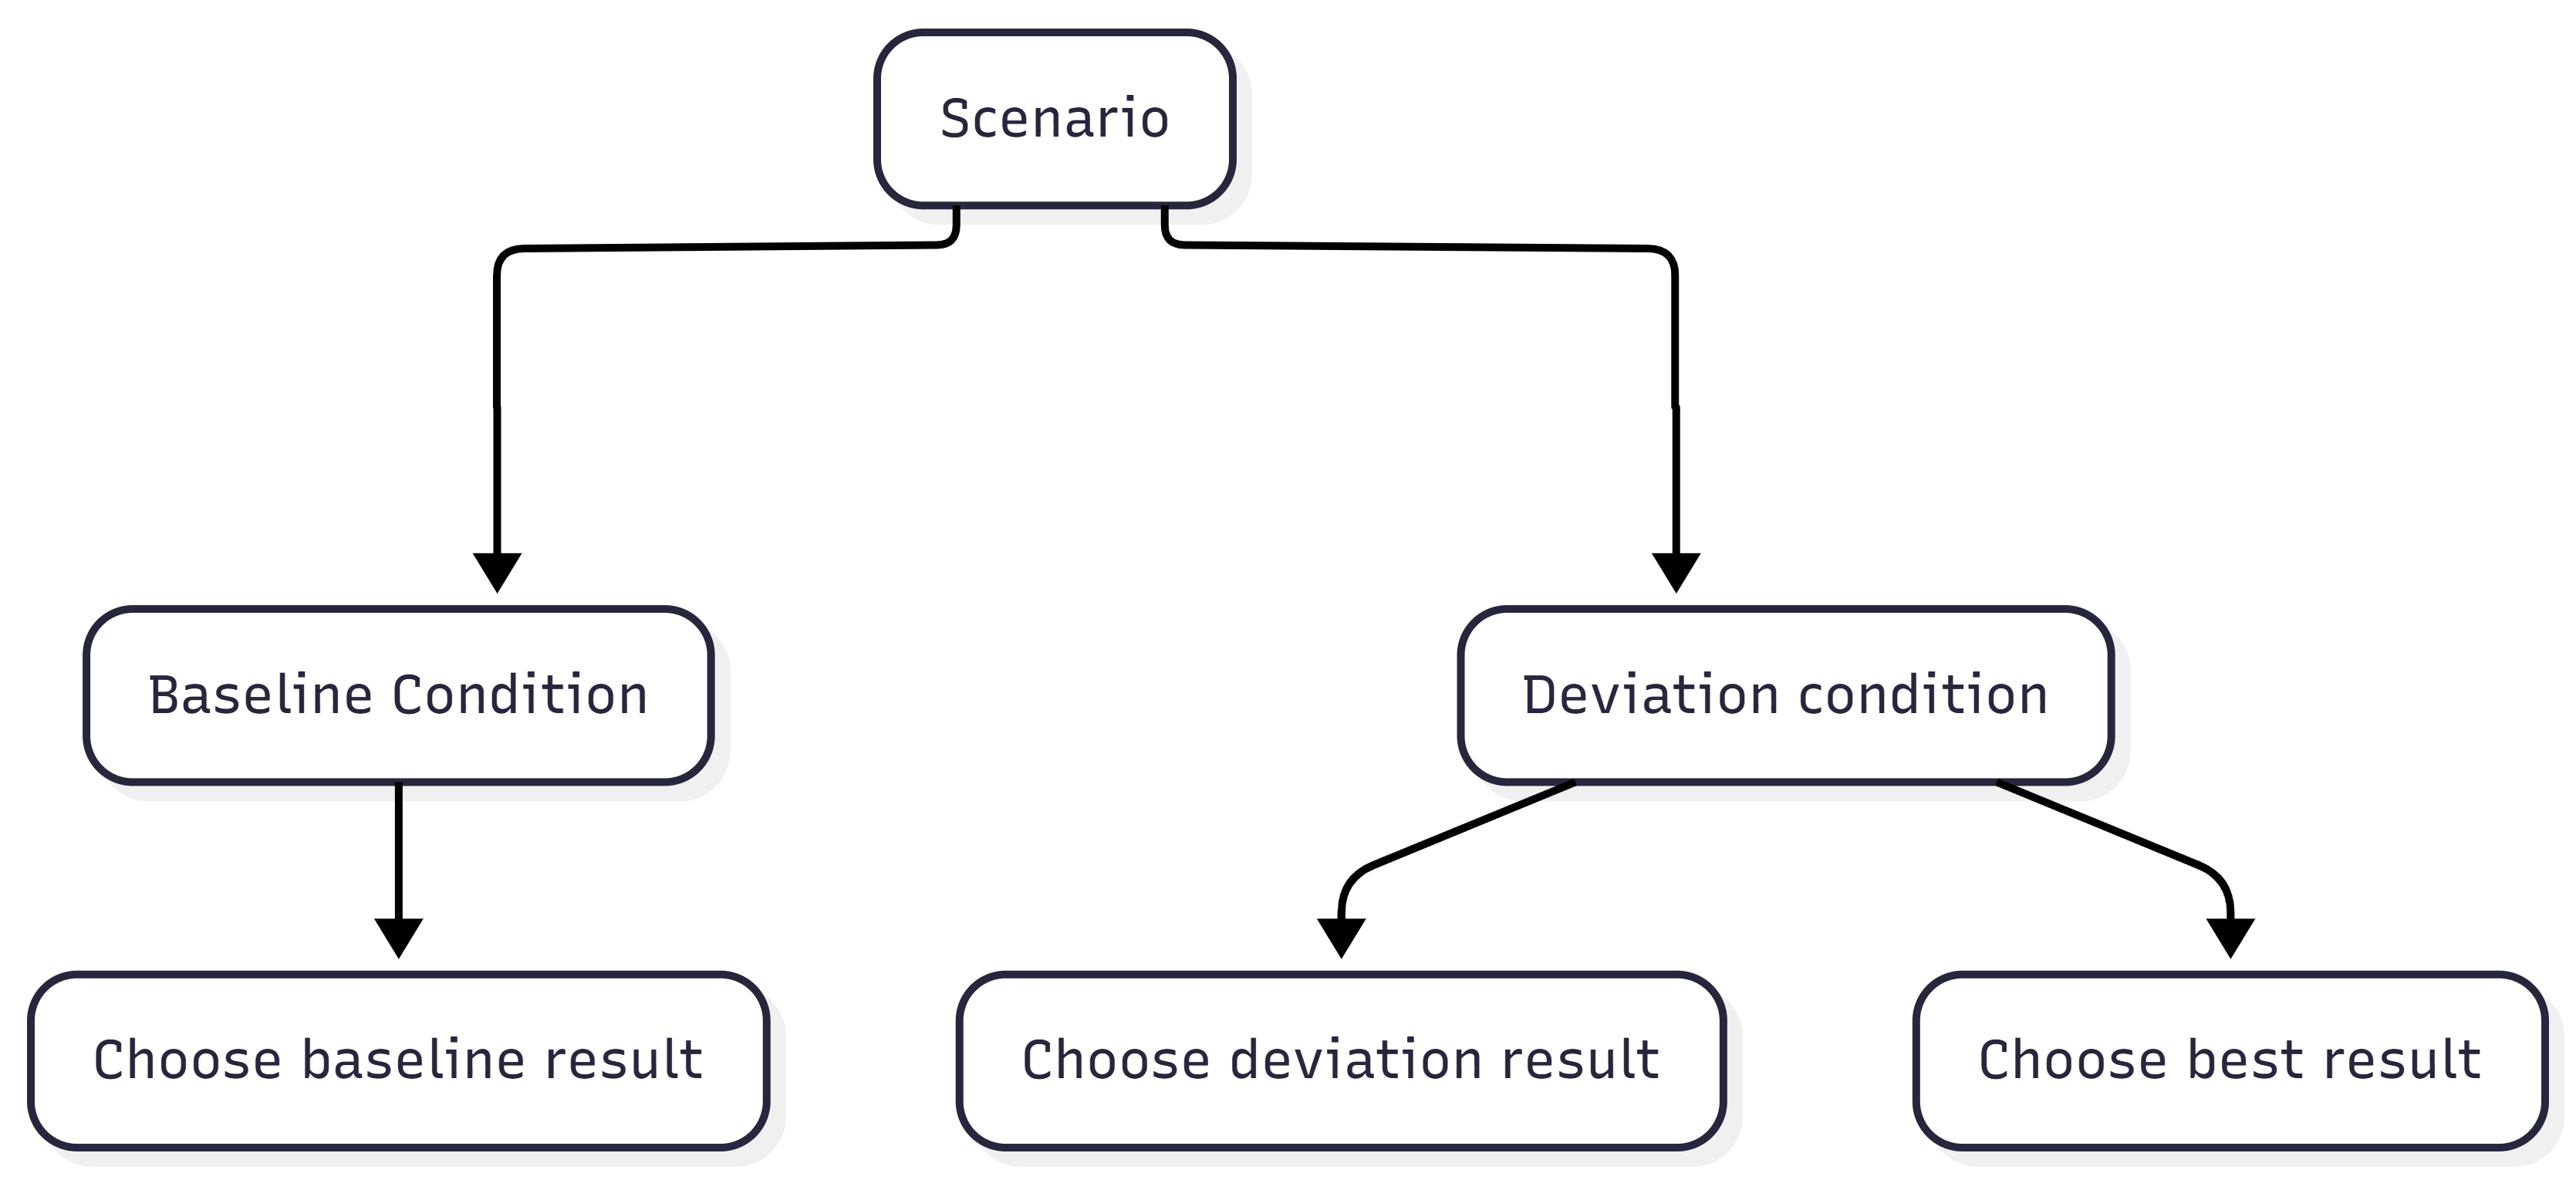
\includegraphics[keepaspectratio]{../Visuals/phases.png}}

}

\caption{\label{fig-phases}Condition Comparisons}

\end{figure}%

\emph{Note.} This figure illustrates the study phases. In phase 1, the
baseline result is compared to the deviation result. In phase 2, the
baseline result is compared to the best result.

\subsubsection{Performance measures}\label{performance-measures}

Performance is assessed through the type I and type II error for the
estimand \(\beta_1\). Specifically, the regression coefficient itself,
the \emph{p}-value and the confidence interval are recorded for each
condition in each repetition.

The type I error refers to a false-positive, or rejecting the
null-hypothesis when it is true. In this study that would mean detecting
an effect in the no-effect scenario. Type I error is generally
acceptable at a rate of 5\% or below, based on an alpha level of .05. In
this case, a rate of higher than 5\% is considered an inflated type I
error rate.

Type II error refers to a false negative, or failing to reject the
null-hypothesis when it is false. In this study that would mean failing
to detect an effect in the effect scenario. Type II error is commonly
assessed in the form of power. Power is \(1-\beta\), where \(\beta\) is
the type II error. The nominal type II error rate of .20 results in a
generally accepted power of 80\%. In this study, type II error will be
expressed in the form of power rates and consequently, power below 80\%
is considered deflated power.

The number of iterations is based on the desired precision of the
project. A Monte-Carlo standard error (MCSE) of 0.01 is deemed
appropriate. According to the formula by Morris et al. (2019), the
required number of iterations to achieve the desired MCSE is 1600
(Equation~\ref{eq-mcsepower}). With an MCSE of 0.01, power rates are
assessed at a precision interval of {[}79, 81{]} around the nominal
power of 80\%. Power levels outside of this range can be stated to have
increased or deflated power levels that are not due to simulation noise.

For the type I error, 1600 iterations results in an MCSE of 0.00545
(Equation~\ref{eq-mcsetypeI}). This means that type I error is assessed
with a precision interval of {[}0.045, 0.055{]} around the nominal
\(\alpha\) level of .05. Any type I error rates outside of this interval
are considered deflated or inflated.

\begin{figure}

\centering{

\begin{figure}[H]

\begin{minipage}{0.50\linewidth}
\begin{equation}\phantomsection\label{eq-mcsepower}{
\begin{aligned}
MCSE &= \sqrt{\frac{\widehat{\text{Power}}\left(1-\widehat{\text{Power}}\right)}{n_{\text{sim}}}},\\
0.01 &= \sqrt{\frac{\widehat{\text{0.8}}\left(1-\widehat{\text{0.8}}\right)}{n_{\text{sim}}}}, \\
n_\text{sim} &= \frac{0.8 \times 0.2}{(0.01)^2},\\
n_\text{sim} &= 1600
\end{aligned}
}\end{equation}\end{minipage}%
%
\begin{minipage}{0.50\linewidth}
\begin{equation}\phantomsection\label{eq-mcsetypeI}{
\begin{aligned}
MCSE &= \sqrt{\frac{\widehat{\text{Type I error}}\left(1-\widehat{\text{Type I error}}\right)}{n_{\text{sim}}}},\\
MCSE &= \sqrt{\frac{\widehat{\text{0.05}}\left(1-\widehat{\text{0.05}}\right)}{1600}}, \\
MCSE &= \sqrt{2.96875e-05},\\
MCSE &= 0.00545
\end{aligned}
}\end{equation}\end{minipage}%

\end{figure}%

}

\caption{\label{fig-mcse}\emph{Note.} Calculations for the number of
iterations based on the desired MCSE for power and the MCSE for type I
error based on the number of iterations.}

\end{figure}%

\subsubsection{Disclosures}\label{disclosures}

\paragraph{Preregistration, reproducibility and
ethics}\label{preregistration-reproducibility-and-ethics}

This project was preregistered on the 31th of March, 2026. The
preregistration can be found at {[}link{]}. In order to prevent ``seed
hacking'', I preregistered a seed which would only become available
after the date of preregistration. An R package was created for this
project under the name \texttt{thepack} in which all functions necessary
to simulate the data can be found. The package is publicly available at
{[}githublink{]}. In order to advance reproducibility, all other files
related to this project are publicly available at {[}github link{]}.
This includes data, code scripts and output files. I made use of
\texttt{renv} to create a reproducible environment in which package
versions and R version are recorded. Instructions on how to reproduce
the findings can be found in the README file on GitHub.

Ethics approval was obtained on October 7th, 2025 from the Utrecht
University faculty of Social Sciences under case-number \#25-1980.

\subsection{Results}\label{results}

\subsubsection{Research question one}\label{research-question-one}

The primary research aim of this study is to examine the effects of
deviations from preregistration on type I and type II errors. In this
section the type I error and power of each deviation condition are
compared to the nominal levels. The Monte Carlo standard error resulted
in a precision range of {[}0.045, 0.055{]} around the nominal type I
error of 0.05 and a range of {[}79,81{]} around the nominal 80\% power.
Values outside of these ranges are considered inflated or deflated.
Figure~\ref{fig-rq1.y} and Figure~\ref{fig-rq1.n} show the type I error
and power for each condition along with the precision range.

\paragraph{Effects on power}\label{effects-on-power}

Within the Sample Size domain, the effects reflect what is known from
the existing literature. Increasing the sample size, increases the power
and decreasing the sample size decreases the power {[}sources{]}. These
effects can be observed in the current study as well
(Figure~\ref{fig-rq1.y}).

Deviations in the Outlier Exclusion Criteria domain also impact power.
When using a strict \emph{z}-score (exclusion based on 2 \emph{SD}
(standard deviation) instead of 3 \emph{SD}) power increases to 83.8\%.
This means that we are able to detect existing effects more often than
in the nominal rate. When using Cook's distance instead of
\emph{z}-scores, the power drops to 68.2\%. This indicates that, when
this method is used, we are less likely to observe an existing effect in
the generated data then we would in the nominal rate. Cook's distance is
generally considered a less conservative form of outlier exclusion
because it only excludes observations based on their influence on the
regression coefficient. It is therefore quite unexpected to see such a
large drop in power in this condition.

In the Statistical Model domain, deflated power is only observed in the
alternative outcome condition. Deviating by using an alternative,
correlated outcome variable resulted in a power of 35.2\%. Both the
continuous and dichotomous covariate conditions have no apparent effect
on power.

This simulation study demonstrates that power can be affected when
researchers are forced to deviate from a preregistration. This effect
can be positive or negative, depending on the type of deviation.
Overall, collecting much fewer participants, using Cook's distance as
outlier criterium and switching to an alternative outcome all deflate
powers. Power is most impacted by switching outcomes, with a steep drop
off from the nominal 80\% to 35.2\% power. Small changes in sample size
and the addition of a covariate show no effect, whereas collecting many
more participants than planned and using a \emph{z}-score of two
standard deviations show slight increases in power.

\begin{figure}

\centering{

\pandocbounded{
\includegraphics[keepaspectratio]{Thesis_files/figure-pdf/fig-rq1.y-1.pdf}}

}

\caption{\label{fig-rq1.y}Power for Baseline and Deviation Conditions in
the Effect scenario}

\end{figure}%

\paragraph{Effects on Type I error}\label{effects-on-type-i-error}

Only two conditions show results outside of the precision range. Small
increases in effect size show an increased type I error of 5.6\%. Using
a strict \emph{z-}score results in a type I error rate of 5.8\%. All
other deviation scenarios fall within the prespecified precision range
and therefore do not indicate any effects on the type I error
(Figure~\ref{fig-rq1.n}).

The small inflation when slightly increasing the sample size is a
borderline case. Using the MCSE of 0.055, which was preregistered for
this study, means that it falls outside of the precision range. Outside
of this range the effects are unlikely to be due to simulation noise.
Using the empirical MCSE of this condition, however, shows that the
found effect might still be due to noise. With a type I error of
0.055625, the empirical MCSE becomes 0.00573. This means that type I
error rates higher than 0.055729 would be considered inflated, which
this condition just remains beneath. In light of this, all other
conditions were also evaluated using the empirical MCSE. The slight
increase in sample size remained the only condition in which this
changed the conclusion.

\begin{figure}

\centering{

\pandocbounded{
\includegraphics[keepaspectratio]{Thesis_files/figure-pdf/fig-rq1.n-1.pdf}}

}

\caption{\label{fig-rq1.n}Type I error rate for Baseline and Deviation
scenarios in the no-effect Scenario}

\end{figure}%

\subsubsection{Research question two}\label{research-question-two}

The second research question pertains to the effect of \emph{choosing}
to deviate when the baseline condition is non-significant. This is done
by comparing an opportunistic scenario to the nominal type I error and
power. In the opportunistic scenario, one condition was recorded per
iteration. Whenever the baseline condition was significant, it was
selected. If the baseline was non-significant, a significant deviation
condition was selected instead, if available, and the number of
significant deviations was recorded. Table~\ref{tbl-rq2} displays how
often significant baselines and significant deviation conditions were
found.

As expected, we observed a positive effect of choosing to deviate on
power. Conditions were selected in order to maximize the number of
significant results, consequently, an increase in power was anticipated.
In 1484 out of 1600 repetitions, a significant condition was observed.
This results in a power of 92.7\% in the effect scenario. In the
no-effect scenario, 261 out of 1600 repetitions showed a significant
condition. Yielding an inflated type I error rate of 16.3\%. This is a
large inflation compared to the nominal level of 5\% and similarly much
higher than the highest type I error rate observed in a singular
deviation condition. The highest type I error rate observed for research
question one was 5.8\% in the Strict z-score condition.

In the effect scenario, 79.9\% of the repetitions resulted in a
significant baseline. Of the 321 repetitions where the baseline was
non-significant, 36.1\% also reported no significant deviation
conditions. The remaining 64\% of repetitions, in which the baseline was
non-significant, had at least one significant deviation, with seven
significant deviation conditions at most.

In the no-effect scenario, the majority (83.7\%) of the repetitions
showed a non-significant baseline as well as non-significant deviations
(Table~\ref{tbl-rq2}).

Significant baseline conditions were observed 5.2\% of the time, which
is in line with the nominal \(\alpha\) level of 5\%. However of the
repetitions in which the baseline was non-significant, 13.3\% showed at
least one significant result. This indicates that when researchers
obtain non-significant results from their preregistered data, and choose
to deviate in one of the investigated ways, they can still find a
significant result 13.3\% of the time. When combining the significant
baseline conditions and significant deviation conditions, the type I
error rate inflated to 16.3\%. This is a large increase in the number of
false positives when picking an available significant result.

\begin{table}

\caption{\label{tbl-rq2}Distribution of the number of significant
deviations (with a non-significant baseline}

\centering{

\centering\begingroup\fontsize{12}{14}\selectfont

\begin{tabular}{lll}
\toprule
\multicolumn{1}{c}{Significant deviation conditions} & \multicolumn{2}{c}{Occurences} \\
\cmidrule(l{3pt}r{3pt}){1-1} \cmidrule(l{3pt}r{3pt}){2-3}
  & Effect & No-effect\\
\midrule
(Significant baseline) & 1279 (79.9\%) & 83 (5.2\%)\\
0 & 116 (7.2\%) & 1339 (83.7\%)\\
1 & 75 (4.7\%) & 126 (7.9\%)\\
2 & 61 (3.8\%) & 27 (1.7\%)\\
3 & 30 (1.9\%) & 17 (1.1\%)\\
\addlinespace
4 & 31 (1.9\%) & 5 (0.3\%)\\
5 & 4 (0.2\%) & 1 (0.1\%)\\
6 & 3 (0.2\%) & 2 (0.1\%)\\
7 & 1 (0.1\%) & 0 (0\%)\\
\bottomrule
\end{tabular}
\endgroup{}

}

\end{table}%

\subsection{Discussion}\label{discussion}

Claesen et al. (2021) and van den Akker, Bakker, et al. (2024) have
shown that deviating from preregistration plans happen very commonly.
The goal of this simulation study was to investigate the effects of
these deviations. In order to do so we identified three main domains in
which deviations commonly occur and put together nine deviation
conditions. These deviations were then examined in terms of their
effects on type I and type II error. The results of the study show that
both are affected by deviations.

\subsubsection{Forced deviations}\label{forced-deviations}

The results of this simulation study show that type I error and power
are both affected when researchers are forced to deviate from a
preregistration. Power can be affected both positively and negatively,
depending on the type of deviation and whether there is an effect to be
detected. This corroborates the idea theorized by Lakens (2024) that it
is not inherently bad to deviate from a preregistration. Power showed
small inflations and deflations, depending on the type of deviation.
Only two deviation conditions showed effects on the type I error. For
all other conditions, effects on type I error were not strong enough to
suggest an effect outside of simulation noise. This shows that there is
little risk of inflating the type I error when being forced to deviate
from a preregistration except for using a stricter \emph{z}-score as
outlier criterium.

Before conducting research, the researcher does not know whether they
will be working with an effect or not. As a result, the researcher
cannot predict whether their deviation will hurt their type I or type II
error. Deviating in the number of standard deviations used to calculate
\emph{z}-scores can positively impact power in an effect scenario yet
inflate type I error in a no-effect scenario. Because the researcher
does not know which scenario they are facing, this type of deviation is
best avoided in order to prevent an inflated type I error rate in the
case of a no-effect scenario.

Consequently, from these results we can conclude that negative impacts
on type I and/or type II can occur when researchers are forced to
deviate by 1) strongly decreasing the sample size, 2) using Cook's
distance as outlier criterium (as opposed to a \emph{z}-score of 3
\emph{SD}), 3) switching to an alternative outcome with a moderate to
high correlation with the original outcome variable, and 4) using a
stricter \emph{z-}score as outlier criterium. These four types of
deviations appear to be most consequential as they can either deflate
power or inflate the type I error.

\subsubsection{Opportunistic deviations}\label{opportunistic-deviations}

The results also showed an effect of deviating opportunistically on the
type I error rate and on power. The type I error rate of 16.3\% in the
opportunistic condition indicates that when researchers choose to make
alterations to their methodology when they find non-significant results,
their risk of reporting false positives becomes much higher.

The types of deviations investigated in this simulation are based on
which deviations are commonly reported. Many other deviations might also
occur, and many deviations might also go unreported. This means that
even in preregistered papers, type I error rates might be even higher
than the 16.3\% found in this study and much higher than the aspired
5\%.

\subsubsection{Limitations}\label{limitations}

It is important to note that the data simulated in this study was based
on one set of parameter values. This is likely to make the results less
generalizable to other disciplines in which the currently used data
structure is less common. The baseline sample size, effect size and
methods investigated are all common among social sciences but might look
much different for other statistics oriented disciplines such as
medicine. It remains unknown whether the found effects would hold up
under smaller and larger samples or effect sizes. Therefore, future
research might explore whether these results persist under alternative
data-generating mechanisms.

Furthermore, opportunistic deviation was limited to singular deviations
in this research, meaning that only one deviation was made at a time,
deviations were not be combined. In vivo, researchers might choose to
deviate in multiple ways simultaneously. Similar to \emph{p}-hacking,
multiple deviation methods might be combined to achieve significant
results. This could lead to even higher type I error rates than found in
this study. These results might therefore underestimate the actual
impact of opportunistic deviations and real type I error rates in
deviation papers might be a lot higher. Further research into this topic
might explore a factorial version of this simulation study to examine
these effects.

\subsubsection{Implications and
conclusions}\label{implications-and-conclusions}

Deviating from a preregistered research plan is not inherently bad. It
can serve to improve or worsen the number of false positives and
negatives depending on the type of deviation and the reason for
deviating. Forced deviations show negative impacts on power and type I
error but might be hard to prevent due to the uncontrollable nature of
the deviation. Choosing to deviate in order to get better results shows
a larger impact on the number of false positives and therefore forms a
bigger issue.

As of yet, researchers often fail to report their reasons for deviating
(Claesen et al., 2021; Willroth \& Atherton, 2024). This is a big issue
when the current results show that choosing to deviate opportunistically
leads to a much larger inflation in the type I error rate than forced
deviations. There has been a call to report deviations from
preregistrations for a while now (Claesen et al., 2021; Heirene et al.,
2024; Willroth \& Atherton, 2024). We suggest going one step further,
and recommend reporting the reasons for the deviation as well. A
deviation template has been proposed by Willroth \& Atherton (2024)
which includes reporting the reasons for deviating. We recommend that
this type of reporting becomes the standard among preregistered papers.
When researchers properly document how they deviate and why they
deviated, it would allow readers to evaluate the possible effects of the
deviations more critically. Readers can then draw their own conclusions
on the validity of the results.

The goal of preregistration is to limit flexibility and improve
reliability of research. The lack of transparency in the reasons for
deviations limits the extent to which these goals can be achieved.
Therefore we recommend that researchers register the reasons for
deviating from their preregistrations. Because deviations are not
inherently bad, but they do have the potential to be harmful.

\textbf{Transparency} \emph{Author Contributions} Anna J. Vijlbrief:
Conceptualization; Methdology; Investigation; Formal Analysis; Software;
Visualization; Writing - original draft; Writing - reviewing and editing
Anne M. Scheel: Conceptualization; Supervision; Writing - reviewing and
editing Hanne I. Oberman: Conceptualization; Supervision; Writing -
reviewing and editing

\emph{Declaration of Conflicting Interests} The author(s) declare that
there were no conflicts of interest with respect to the authorship or
the publication of this article.

\newpage

\subsection*{References}\label{references}
\addcontentsline{toc}{subsection}{References}

\phantomsection\label{refs}
\begin{CSLReferences}{1}{0}
\bibitem[\citeproctext]{ref-bakker2014}
Bakker, M., \& Wicherts, J. M. (2014). Outlier {Removal} and the
{Relation} with {Reporting Errors} and {Quality} of {Psychological
Research}. \emph{PLOS ONE}, \emph{9}(7), e103360.
\url{https://doi.org/10.1371/journal.pone.0103360}

\bibitem[\citeproctext]{ref-brodeur2024}
Brodeur, A., Cook, N. M., Hartley, J. S., \& Heyes, A. (2024). Do
{Preregistration} and {Preanalysis Plans Reduce} {\emph{p}} -{Hacking}
and {Publication Bias}? {Evidence} from 15,992 {Test Statistics} and
{Suggestions} for {Improvement}. \emph{Journal of Political Economy
Microeconomics}, \emph{2}(3), 527--561.
\url{https://doi.org/10.1086/730455}

\bibitem[\citeproctext]{ref-claesen2021}
Claesen, A., Gomes, S., Tuerlinckx, F., \& Vanpaemel, W. (2021).
Comparing dream to reality: An assessment of adherence of the first
generation of preregistered studies. \emph{Royal Society Open Science},
\emph{8}(10), 211037. \url{https://doi.org/10.1098/rsos.211037}

\bibitem[\citeproctext]{ref-ferguson2023}
Ferguson, J., Littman, R., Christensen, G., Paluck, E. L., Swanson, N.,
Wang, Z., Miguel, E., Birke, D., \& Pezzuto, J.-H. (2023). Survey of
open science practices and attitudes in the social sciences.
\emph{Nature Communications}, \emph{14}(1), 5401.
\url{https://doi.org/10.1038/s41467-023-41111-1}

\bibitem[\citeproctext]{ref-heirene2024}
Heirene, R., LaPlante, D., Louderback, E., Keen, B., Bakker, M.,
Serafimovska, A., \& Gainsbury, S. (2024). Preregistration specificity
and adherence: {A} review of preregistered gambling studies and
cross-disciplinary comparison. \emph{Meta-Psychology}, \emph{8}.
\url{https://doi.org/10.15626/MP.2021.2909}

\bibitem[\citeproctext]{ref-john2012}
John, L. K., Loewenstein, G., \& Prelec, D. (2012). Measuring the
{Prevalence} of {Questionable Research Practices With Incentives} for
{Truth Telling}. \emph{Psychological Science}, \emph{23}(5), 524--532.
\url{https://doi.org/10.1177/0956797611430953}

\bibitem[\citeproctext]{ref-lakens2024}
Lakens, D. (2024). When and {How} to {Deviate From} a {Preregistration}.
\emph{Collabra: Psychology}, \emph{10}(1), 117094.
\url{https://doi.org/10.1525/collabra.117094}

\bibitem[\citeproctext]{ref-leys2013}
Leys, C., Ley, C., Klein, O., Bernard, P., \& Licata, L. (2013).
Detecting outliers: {Do} not use standard deviation around the mean, use
absolute deviation around the median. \emph{Journal of Experimental
Social Psychology}, \emph{49}(4), 764--766.
\url{https://doi.org/10.1016/j.jesp.2013.03.013}

\bibitem[\citeproctext]{ref-lindsay2018}
Lindsay, S. D., Nosek, B. A., \& Stephen, D. (2018). Preregistration
{Becoming} the {Norm} in {Psychological Science}. \emph{APS Observer},
\emph{31}.

\bibitem[\citeproctext]{ref-morris2019a}
Morris, T. P., White, I. R., \& Crowther, M. J. (2019). Using simulation
studies to evaluate statistical methods. \emph{Statistics in Medicine},
\emph{38}(11), 2074--2102. \url{https://doi.org/10.1002/sim.8086}

\bibitem[\citeproctext]{ref-opensciencecollaboration2015}
Open Science Collaboration. (2015). Estimating the reproducibility of
psychological science. \emph{Science}, \emph{349}(6251), aac4716.
\url{https://doi.org/10.1126/science.aac4716}

\bibitem[\citeproctext]{ref-rcoreteam2024}
R Core Team. (2024). \emph{R: {A Language} and {Environment} for
{Statistical Computing}}. R Foundation for Statistical Computing.

\bibitem[\citeproctext]{ref-simmons2011}
Simmons, J. P., Nelson, L. D., \& Simonsohn, U. (2011). False-{Positive
Psychology}: {Undisclosed Flexibility} in {Data Collection} and
{Analysis Allows Presenting Anything} as {Significant}.
\emph{Psychological Science}, \emph{22}(11), 1359--1366.
\url{https://doi.org/10.1177/0956797611417632}

\bibitem[\citeproctext]{ref-stefan2023}
Stefan, A. M., \& Schönbrodt, F. D. (2023). \emph{Big little lies: A
compendium and simulation of p-hacking strategies}.

\bibitem[\citeproctext]{ref-vandenakker2024}
van den Akker, O. R., Bakker, M., Van Assen, M. A. L. M., Pennington, C.
R., Verweij, L., Elsherif, M. M., Claesen, A., Gaillard, S. D. M.,
Yeung, S. K., Frankenberger, J.-L., Krautter, K., Cockcroft, J. P.,
Kreuer, K. S., Evans, T. R., Heppel, F. M., Schoch, S. F., Korbmacher,
M., Yamada, Y., Albayrak-Aydemir, N., \ldots{} Wicherts, J. M. (2024).
The potential of preregistration in psychology: {Assessing}
preregistration producibility and preregistration-study consistency.
\emph{Psychological Methods}. \url{https://doi.org/10.1037/met0000687}

\bibitem[\citeproctext]{ref-vandenakker2024a}
van den Akker, O. R., van Assen, M. A. L. M., Bakker, M., Elsherif, M.,
Wong, T. K., \& Wicherts, J. M. (2024). Preregistration in practice: {A}
comparison of preregistered and non-preregistered studies in psychology.
\emph{Behavior Research Methods}, \emph{56}(6), 5424--5433.
\url{https://doi.org/10.3758/s13428-023-02277-0}

\bibitem[\citeproctext]{ref-willroth2024}
Willroth, E. C., \& Atherton, O. E. (2024). \emph{Best {Laid Plans}: {A
Guide} to {Reporting Preregistration Deviations}}.

\end{CSLReferences}




\end{document}
